\let\negmpace\undefined
\let\negthickspace\undefined
\documentclass[journal]{IEEEtran}
\usepackage[a5paper, margin=10mm, onecolumn]{geometry}
%\usepackage{lmodern} % Ensure lmodern is loaded for pdflatex
% Include tfrupee package
\setlength{\headheight}{1cm} % Set the height of the header box
\setlength{\headsep}{0mm}     % Set the distance between the header box and the top of the text
\usepackage{xparse}
\usepackage{gvv-book}
\usepackage{gvv}
\usepackage{cite}

\usepackage{amsmath,amssymb,amsfonts,amsthm}
\usepackage{algorithmic}
\usepackage{graphicx}
\usepackage{textcomp}
\usepackage{xcolor}
\usepackage{txfonts}
\usepackage{listings}
\usepackage{enumitem}
\usepackage{mathtools}
\usepackage{gensymb}
\usepackage{comment}
\usepackage[breaklinks=true]{hyperref}
\usepackage{tkz-euclide} 
\usepackage{listings}
% \usepackage{gvv}                                        
\def\inputGnumericTable{}                                 
\usepackage[latin1]{inputenc}                                
\usepackage{color}                                            
\usepackage{array}                                            
\usepackage{longtable}                                       
\usepackage{calc}                                             
\usepackage{multirow}                                         
\usepackage{hhline}                                           
\usepackage{ifthen}                                           
\usepackage{lscape}
\renewcommand{\thefigure}{\theenumi}
\renewcommand{\thetable}{\theenumi}
\setlength{\intextsep}{10pt} % Space between text and floats
\numberwithin{equation}{enumi}
\numberwithin{figure}{enumi}
\renewcommand{\thetable}{\theenumi}
\begin{document}
\bibliographystyle{IEEEtran}
\title{12.8.1.2}
\author{EE24BTECH11033 - KOLLURU SURAJ}
% \maketitle
% \newpage
% \bigskip
{\let\newpage\relax\maketitle}
\textbf{Question:} 
Find the area of the region bounded by $y^2=9x$, $x=2$, $x=4$ and the x-axis in the first quadrant.
\\\\
\solution\\
If the area is calulated directly using integration it would be 
\begin{align}
     A= \int_{2}^{4} 3\sqrt{x}dx\\
     A=\sbrak{3\cdot \frac{2}{3} x^{3/2}}_2^4\\
     A =10.343146
\end{align}
Let's try to verify this computationally using Trapezoidal rule\\
\textbf{Some theory about Trapezoidal rule:}\\
The idea behind the trapezoidal rule is to approximate the region under the curve of the function as a series of trapezoids, rather than using rectangles. The area of each trapezoid is then computed and summed to estimate the total area under the curve (the integral).
First we need to set up the integral\\
Area under curve is given by
\begin{align}
    A= \int_{2}^{4} 3\sqrt{x}dx
\end{align}

We will approximate this using trapezoidal rule. Divide the interval [2,4] into 100 subintervals with each of width $h=\frac{4-2}{100}=\frac{1}{50}$, Let:
\begin{align}
x_0=2,x_1=x_0+h,x_2=x_1+h,....x_n=4
\end{align}
The trapezoidal rule for approximating the integral becomes:

\begin{align}
    A \approx\frac{h}{2}[f(x_0)+ 2\sum_{i=1}^{n-1} f(x_i) +f(x_n)]\label{1}
\end{align}
where $f(x)= \sqrt{3}x$. Substituting it in \ref{1} gives
\begin{align}
     A \approx\frac{3h}{2}[\sqrt{x_0}+ 2\sum_{a=1}^{n-1} \sqrt{x_i} +\sqrt{x_n}]
\end{align}
This is a difference equation because it expresses the total area A as a sum of terms at discrete points $x_i$, with a recurrence-like structure for the summation.\\
Using a C code to find the area using trapezoidal rule, The area is
\begin{align}
    A\approx 10.343135
\end{align}

which appears to be very close to the area we got from the trapezoidal rule.
\begin{figure}[!ht]
    \centering
    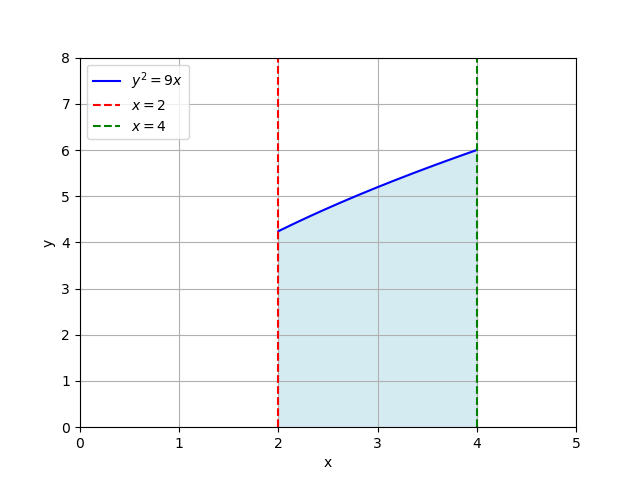
\includegraphics[width=\columnwidth]{figs/Figure_1.png}
    \caption{}
\end{figure}


\end{document}
